\documentclass[xetex,mathserif,serif]{beamer}
\usepackage{polyglossia}
\setdefaultlanguage[babelshorthands=true]{russian}
\usepackage{minted}
\usepackage{tabu}

\useoutertheme{infolines}

\usepackage{fontspec}
\setmainfont{FreeSans}
\newfontfamily{\russianfonttt}{FreeSans}

\setbeamertemplate{blocks}[rounded][shadow=false]

\setbeamercolor*{block title alerted}{fg=red!50!black,bg=red!20}
\setbeamercolor*{block body alerted}{fg=black,bg=red!10}

\tabulinesep=0.7mm

\title{Диаграммы классов UML}
\author[Юрий Литвинов]{Юрий Литвинов \newline \textcolor{gray}{\small\texttt{yurii.litvinov@gmail.com}}}

\date{04.03.2020г}

\begin{document}
	
	\frame{\titlepage}

	\section{CI}

	\begin{frame}
		\frametitle{Ликбез по Continuous Integration}
		Непрерывная интеграция --- практика слияния всех изменений по нескольку раз в день, сборки их в известном окружении и запуска юнит-тестов.
		\begin{itemize}
			\item Автоматический билд
			\begin{itemize}
				\item Всё, что нужно для сборки, есть в репозитории, может быть получено на чистую (ну, практически) машину и собрано одной консольной командой
			\end{itemize}
			\item Большое количество юнит-тестов, запускаемых автоматически
			\item Выделенная машина, слушающая репозиторий и выполняющая билд
			\begin{itemize}
				\item Чаще всего каждый билд запускается на заранее настроенной виртуалке
			\end{itemize}
		\end{itemize}
	\end{frame}

	\begin{frame}
		\frametitle{Continuous Integration}
		\begin{itemize}
			\item Извещение всех разработчиков о статусе
			\begin{itemize}
				\item Если билд не прошёл, разработка приостанавливается до его починки
			\end{itemize}
			\item Автоматическое выкладывание
			\item Пока билд не прошёл, задача не считается сделанной
			\begin{itemize}
				\item Короткие билды (<10 мин.)
				\item deployment pipeline
				\begin{itemize}
					\item Отдельная машина для сборки, для коротких тестов, для длинных тестов, для выкладывания
				\end{itemize}
			\end{itemize}
		\end{itemize}
	\end{frame}

	\subsection{Travis}

	\begin{frame}
		\frametitle{Travis}
		\begin{itemize}
			\item \url{https://travis-ci.org/} --- пример бесплатной для open source-проектов облачной CI-системы
			\item Собирает на чистой виртуальной машине под Ubuntu 12.04, 14.04, 16.04 или OS X 10.13 (есть экспериментальная поддержка Windows)
			\item Интегрируется с GitHub-ом, Slack-ом, умеет деплоить
			\item Окружение настраивается конфигурационным файлом или ``вручную'' из скрипта сборки (некоторые конфигурации разрешают sudo)
			\item Сборка выполняется либо автоматически, либо указанным скриптом сборки
			\item Build Matrix
			\begin{itemize}
				\item Разные конфигурации сборки, выполняемые на разных виртуальных машинах
			\end{itemize}
		\end{itemize}
	\end{frame}

	\begin{frame}
		\frametitle{Travis, настройка сборки}
		\begin{itemize}
			\item Установить commit hook на гитхабе
			\begin{itemize}
				\item Travis умеет это делать сам, надо залогиниться под своим GitHub-аккаунтом на Travis и выбрать нужный репозиторий в профиле
			\end{itemize}
			\item Добавить .travis.yml в корень репозитория
			\begin{itemize}
				\item Это конфигурационный файл, говорящий, что и как собирать
			\end{itemize}
			\item Закоммитить и запушить, это инициирует процесс сборки
			\begin{itemize}
				\item Коммит, где в комментарии есть подстрока ``[ci skip]'', игнорируется Travis-ом, остальные он собирает
			\end{itemize}
			\item Результаты будут видны у каждого коммита в истории и в пуллреквесте
		\end{itemize}
		\begin{center}
			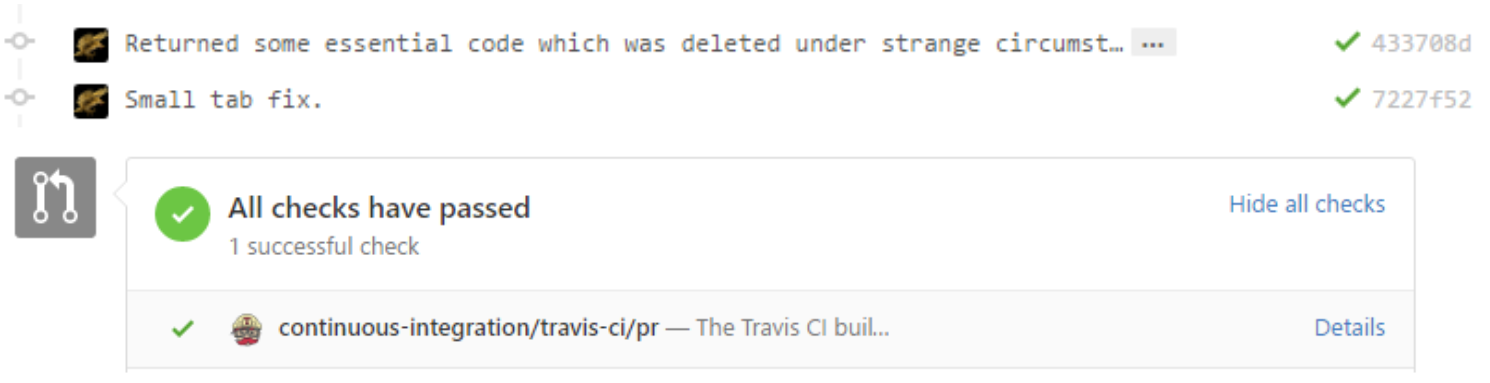
\includegraphics[width=0.7\textwidth]{travisSuccess.png}
		\end{center}
	\end{frame}

	\begin{frame}[fragile]
		\frametitle{Travis, конфигурационный файл}
		\begin{minted}{yaml}
language: java
		\end{minted}
		--- всё :) Если у вас проект прямо в корне репозитория.

		Жизненный цикл сборки:
		\begin{footnotesize}
			\begin{itemize}
				\item Install apt addons
				\item before\_install
				\item install
				\item before\_script
				\item script
				\item after\_success или after\_failure
				\item \mintinline{text}|[OPTIONAL]| before\_deploy
				\item \mintinline{text}|[OPTIONAL]| deploy
				\item \mintinline{text}|[OPTIONAL]| after\_deploy
				\item after\_script
			\end{itemize}
		\end{footnotesize}
	\end{frame}

	\begin{frame}
		\frametitle{Travis, примеры}
		\begin{itemize}
			\item Веб-приложение из нескольких сервисов на Java:
			\begin{itemize}
				\item \url{https://github.com/qreal/wmp/blob/master/.travis.yml}
			\end{itemize}
			\item Относительно большое десктопное приложение на C++:
			\begin{itemize}
				\item \url{https://github.com/qreal/qreal/blob/master/.travis.yml}
			\end{itemize}
			\item Билд в Docker-окружении (все зависимости носим с собой):
			\begin{itemize}
				\item \url{https://github.com/trikset/trikRuntime/blob/master/.travis.yml}
			\end{itemize}
		\end{itemize}
	\end{frame}

	\begin{frame}[fragile]
		\frametitle{Travis, пример конфига для домашки}
		\begin{minted}{yaml}
language: java
os:
  - linux
env:
  - PROJECT_DIR=hw1
  - PROJECT_DIR=hw2
  - PROJECT_DIR=hw3
script: cd $PROJECT_DIR && ./gradlew check
		\end{minted}
	\end{frame}

	\subsection{AppVeyor}

	\begin{frame}
		\frametitle{AppVeyor}
		\begin{itemize}
			\item CI c поддержкой Windows и Linux, прежде всего для сборки .NET-приложений, но умеет много чего ещё
			\begin{itemize}
				\item Windows Server 2016 или Windows Server 2012 R2
				\item Ubuntu 16.04.4 LTS или Ubuntu 18.04 LTS
			\end{itemize}
			\item Тоже бесплатен для open source
			\item Конфигурируется через appveyor.yml
			\item Собирает по умолчанию MSBuild
			\begin{itemize}
				\item Можно переубедить
			\end{itemize}
			\item Синтаксис .yml-файла: \url{https://www.appveyor.com/docs/appveyor-yml/}
			\item Пример: \url{https://github.com/qreal/qreal/blob/master/appveyor.yml}
			\begin{itemize}
				\item Собирать двумя CI-серверами один проект не зазорно
			\end{itemize}
		\end{itemize}
	\end{frame}

	\section{CASE-системы}

	\begin{frame}
		\frametitle{Computer-Aided Software Engineering}
		\begin{itemize}
			\item В 80-е годы термином CASE называли всё, что помогает разрабатывать ПО с помощью компьютера
			\begin{itemize}
				\item Даже текстовые редакторы
			\end{itemize}
			\item Теперь --- прежде всего средства для визуального моделирования (UML-диаграммы, ER-диаграммы и т.д.)
			\item Отличаются от графических редакторов тем, что ``понимают'', что в них рисуют
			\item Нынче чаще используются термины ``MDE tool'', ``UML tool'' и т.д.
			\item Репозиторий + набор визуальных редакторов + генераторы + средства обратного проектирования + иногда много чего ещё
		\end{itemize}
	\end{frame}

	\begin{frame}
		\frametitle{Примеры CASE-инструментов}
		\begin{itemize}
			\item ``Рисовалки''
			\begin{itemize}
				\item Visio
				\item Dia
				\item SmartDraw
				\item Creately
			\end{itemize}
			\item Полноценные CASE-системы
			\begin{itemize}
				\item Enterprise Architect
				\item Rational Software Architect
				\item MagicDraw
				\item Visual Paradigm
				\item GenMyModel
			\end{itemize}
			\item Забавные штуки
			\begin{itemize}
				\item \url{https://www.websequencediagrams.com/}
				\item \url{http://yuml.me/}
				\item \url{http://plantuml.com/}
			\end{itemize}
		\end{itemize}
	\end{frame}

	\section{Диаграммы классов и объектов UML}

	\begin{frame}
		\frametitle{Диаграммы классов UML}
		\begin{center}
			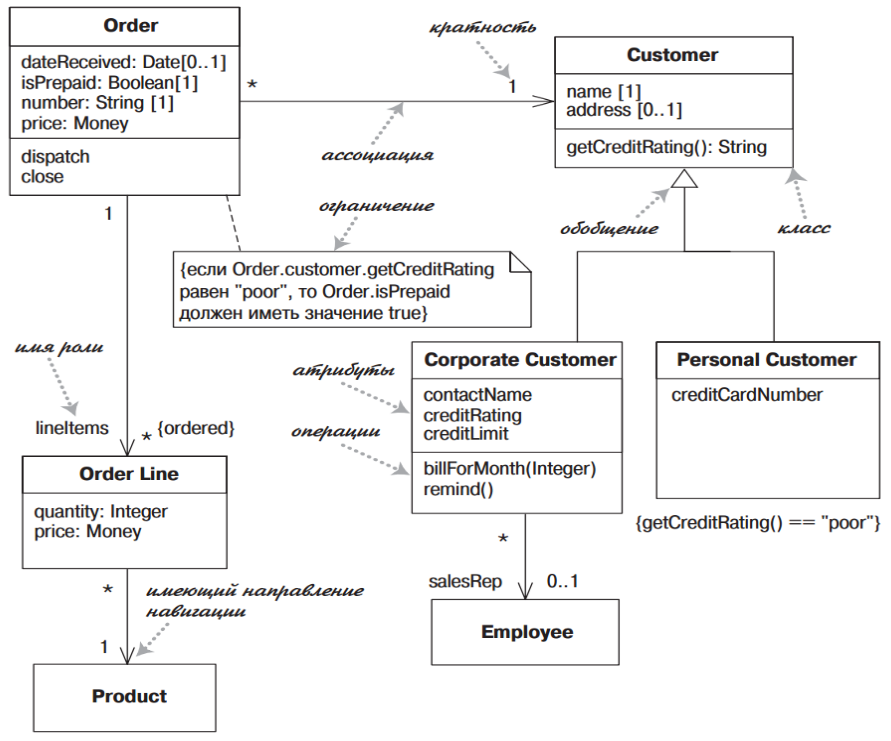
\includegraphics[width=0.7\textwidth]{umlClassDiagram.png}
		\end{center}
	\end{frame}

	\begin{frame}
		\frametitle{Свойства}
		\begin{columns}
			\begin{column}{0.3\textwidth}
				\begin{center}
					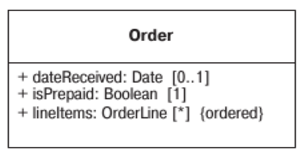
\includegraphics[width=0.8\textwidth]{attributes.png}

					Атрибуты
				\end{center}
			\end{column}
			\begin{column}{0.7\textwidth}
				\begin{center}
					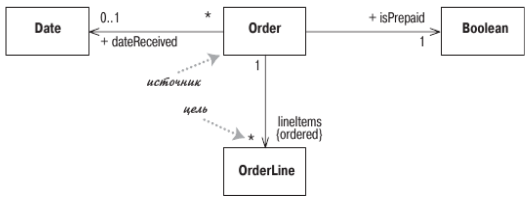
\includegraphics[width=0.7\textwidth]{associations.png}

					Ассоциации
				\end{center}
			\end{column}
		\end{columns}
		\bigskip
		Синтаксис:
		\begin{itemize}
			\item видимость имя: тип кратность = значение по умолчанию \{строка свойств\}
			\item Видимость: + (public), - (private), \# (protected), \char`~ (package)
			\item Кратность: 1 (ровно 1 объект), 0..1 (ни одного или один),\newline * (сколько угодно), 1..*, 2..*
		\end{itemize}
	\end{frame}

	\begin{frame}
		\frametitle{Агрегация и композиция}
		Агрегация – объект ``знает'' о другом (не управляет его временем жизни, имеет на него ссылку или указатель)
		\begin{center}
			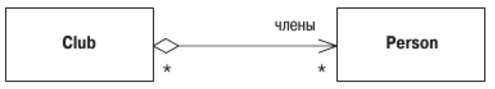
\includegraphics[width=0.5\textwidth]{aggregations.png}
		\end{center}
		Композиция --- объект владеет другим объектом (управляет его временем жизни, хранит его по значению или по указателю, делая delete)
		\begin{center}
			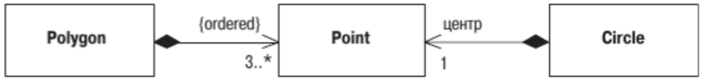
\includegraphics[width=0.7\textwidth]{compositions.png}
		\end{center}
		Уточнение обычной ассоциации, используется только если очень надо
	\end{frame}

	\begin{frame}
		\frametitle{Прочее}
		\begin{columns}
			\begin{column}{0.5\textwidth}
				\begin{center}
					Интерфейсы

					\bigskip
					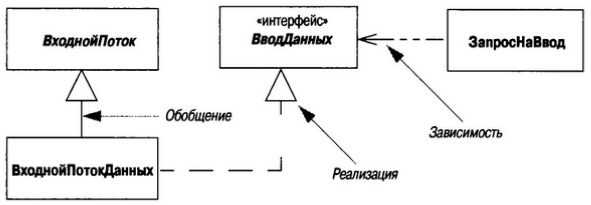
\includegraphics[width=0.9\textwidth]{interfaces1.png}

					\bigskip
					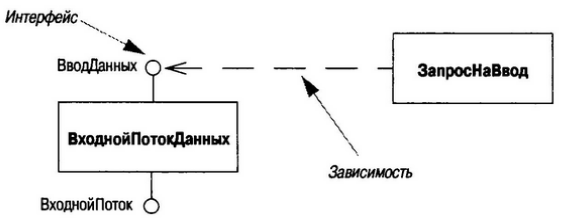
\includegraphics[width=0.9\textwidth]{interfaces2.png}
				\end{center}
			\end{column}
			\begin{column}{0.5\textwidth}
				\begin{center}
					Зависимости

					\bigskip
					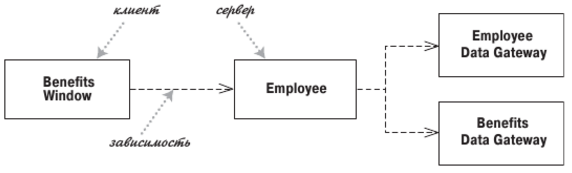
\includegraphics[width=0.9\textwidth]{dependencies.png}
					\bigskip

					Шаблоны

					\bigskip
					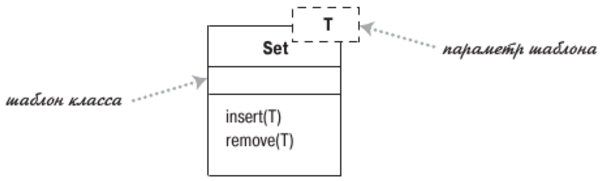
\includegraphics[width=0.9\textwidth]{templates.png}
				\end{center}
			\end{column}
		\end{columns}
	\end{frame}

	\begin{frame}
		\frametitle{Диаграммы объектов}
				\begin{columns}
			\begin{column}{0.5\textwidth}
				\begin{itemize}
					\item snapshot структуры классов во время выполнения
					\item Используются обычно чтобы пояснить диаграмму классов
					\item Полезны на этапе анализа предметной области, ещё до диаграмм классов
				\end{itemize}
			\end{column}
			\begin{column}{0.5\textwidth}
				\begin{center}
					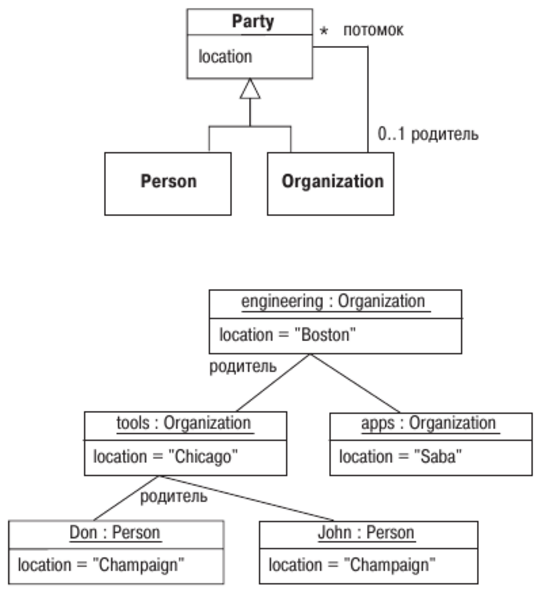
\includegraphics[width=\textwidth]{objectsDiagram.png}
				\end{center}
			\end{column}
		\end{columns}
	\end{frame}

	\section{Задания}

	\begin{frame}
		\frametitle{Домашнее задание: cd, ls}
		\begin{itemize}
			\item Реализовать команды \textbf{ls} и \textbf{cd} на базе кода одногруппника
			\begin{itemize}
				\item Обе команды могут принимать 0 или 1 аргумент
				\item Не забывайте про юнит-тесты
			\end{itemize}
			\item Написать ревью на архитектуру оного одногруппника, указав, что оказалось удобным, а что неудобным при реализации, что можно было бы улучшить
			\item Сделать fork на GitHub, выложить изменения туда и сделать пуллреквест в свой форк
			\begin{itemize}
				\item Если ``жертва'' не против, можно и в исходный репозиторий
			\end{itemize}
			\item Реализация, в которой надо сделать команды, определяется циклическим сдвигом на \textbf{2} вверх по списку на HwProj, с пропуском несданных решений
			\item Дедлайн: \textbf{10:00 18.03.2020г}.
		\end{itemize}
	\end{frame}

	\begin{frame}
		\frametitle{Задание на остаток пары}
		\begin{itemize}
			\item Нарисовать диаграмму классов UML для своего решения CLI, как оно есть
			\item Обращать внимание на синтаксис UML и читаемость диаграммы
			\item Как будет готово, позвать меня и показать
			\item Не пытаться рисовать методы, кроме самых важных
			\item Не рисовать все поля, можно даже не рисовать все классы --- надо успеть до конца пары
		\end{itemize}
	\end{frame}

\end{document}
